\documentclass[10pt]{article}
\usepackage[letterpaper,margin=0.75in]{geometry}
\usepackage{graphicx}
\usepackage{booktabs}
\usepackage{amsmath}
\usepackage{xcolor}
\usepackage{listings}
\usepackage{enumitem}
\usepackage[hidelinks]{hyperref}
\usepackage{caption}
\usepackage{float}
\captionsetup{font=small,labelfont=bf}
\setlist{nosep,leftmargin=1.4em}
\setlength{\parskip}{3pt}
\setlength{\parindent}{0pt}
\lstset{basicstyle=\ttfamily\footnotesize,columns=fullflexible,frame=single,framerule=0.3pt,
        rulecolor=\color{gray!60},xleftmargin=2pt,xrightmargin=2pt,aboveskip=4pt,belowskip=2pt}
\newcommand{\code}[1]{\texttt{#1}}
\graphicspath{{om/figs/}}

% ---------------------------------------------------------------------------
% PLACEHOLDERS. Each orange box is one teammate's part. Replace the box with
% your text (delete the \todo{...}{...} call). To check nothing is left:
%   grep -n todo design_report.tex
% To hide all remaining boxes in a draft: change the definition below to
%   \newcommand{\todo}[2]{}
% Page budget (handout: 3 to 4 pages): about 1 page shared material plus
% roughly 1 page per kernel, so keep each kernel's part to ~1 page.
% ---------------------------------------------------------------------------
\definecolor{todoline}{HTML}{EB6834}
\newcommand{\todo}[2]{\par\noindent\fcolorbox{todoline}{todoline!7}{\parbox{\dimexpr\linewidth-2\fboxsep-2\fboxrule\relax}{\small\textbf{TODO (#1):} #2}}\par}

\title{\vspace{-1.6em}\textbf{Fast Direct Convolution for YOLOv8n on Broadwell}\\[2pt]
\large Mid-project design document: kernel design and implementation}
\author{Om Tank, O'Malley Sherlock, Bohan (Simon) Yu\\
18-645 How to Write Fast Code I, Fall 2026}
\date{\vspace{-1.2em}}

\begin{document}
\maketitle

\noindent We write FP32 kernels for the convolution layers of the pretrained YOLOv8n detector and compare them with OpenCV DNN (our baseline) and ONNX Runtime, on the same ONNX model and the same images. The ONNX export folds BatchNorm into each convolution's weights and bias, so every layer is a convolution plus bias plus SiLU. YOLOv8n has three kinds of convolution, and each of us owns one (Table~\ref{tab:split}). All three kernels share one data layout (Section~\ref{sec:mem}) and one test harness that checks every kernel against the baseline model's own outputs on real images (max relative error $\le 10^{-4}$). Numbers are from ece028, batch 1, single core unless stated otherwise.

\begin{table}[H]\centering\small
\begin{tabular}{p{4.1cm}p{7.2cm}lrr}
\toprule
Kernel & Where in YOLOv8n & Owner & Layers & Share of FLOPs\\
\midrule
3$\times$3 conv, stride 1 & both convs of every C2f bottleneck; first two convs of each Detect branch & Om & 32 & 66\%\\
3$\times$3 conv, stride 2 & the downsampling convs (backbone and neck) & O'Malley & 7 & 15\%\\
1$\times$1 conv; SPPF max-pool; SiLU & start/end of every C2f, SPPF, last conv of each Detect branch & Simon & 24 & 19\%\\
\bottomrule
\end{tabular}
\caption{Kernels and owners. 8.74 GFLOP per 640$\times$640 image in total.}\label{tab:split}
\end{table}

% ===========================================================================
\section{Kernel description}

\subsection{3$\times$3 stride-1 convolution (Om)}
For each image $n$, output channel $k$ and output pixel $(h,w)$:
\[ y_{n,k,h,w} = \mathrm{SiLU}\Big(b_k + \textstyle\sum_{c=0}^{C-1}\sum_{r=0}^{2}\sum_{s=0}^{2} x_{n,c,h+r-1,w+s-1}\, W_{k,c,r,s}\Big). \]
\begin{itemize}
\item \textbf{Independent operations.} Every output element is an independent dot product of length $9C$; a layer has $K\cdot H\cdot W$ of them (25{,}600 to 512{,}000 here).
\item \textbf{Dependent instructions.} Inside one output, a chain of $9C$ fused multiply-adds into one accumulator (144 to 2{,}304 long). With SIMD, 8 output channels share one chain in one register.
\item \textbf{Functional units.} FMA on ports 0 and 1; weight loads and input broadcasts on ports 2 and 3; one store per output vector on port 4; the SiLU epilogue uses the FMA/multiply units and the divider.
\item \textbf{SIMD.} AVX2 with FMA3: 16 YMM registers of 8 FP32 lanes (\code{vfmadd231ps}, \code{vbroadcastss}).
\item \textbf{Specialized units.} None for FP32: no AVX-512, and VNNI/AMX (int8/bf16) are not on this CPU.
\end{itemize}

\subsection{3$\times$3 stride-2 convolution (O'Malley)}
\todo{O'Malley}{Same five bullets for the stride-2 kernel. Layers: \code{model.0, 1, 3, 5, 7, 16, 19} (\code{docs/LAYERS.md}, kind \code{3x3s2}). The formula is the one above with input pixel $(2h+r-1,\,2w+s-1)$, so the output is half the width and height. Independent operations: $K\cdot OH\cdot OW$ outputs per layer. Chain length $9C$. Note the stem \code{model.0}: $C=3$ is padded to one 8-channel block, so 5/8 of its FMA lanes multiply zeros.}

\subsection{1$\times$1 convolution, SPPF max-pool and SiLU (Simon)}
\todo{Simon}{Same five bullets for each of the three. 1$\times$1: $y_{k,p} = b_k + \sum_c x_{c,p} W_{k,c}$ for every pixel $p$, i.e.\ a matrix multiply of [pixels $\times$ C] by [C $\times$ K]; chain length $C$; 24 layers, kind \code{1x1}. SPPF (\code{model.9}): three chained 5$\times$5 stride-1 max-pools on 128 channels at 20$\times$20; independent per output; each pooled output is a chain of 24 \code{vmaxps} over its 5$\times$5 window (8 if done separably), unit = vector ALU, no FLOPs in the FMA sense. SiLU: $x/(1+e^{-x})$ applied to every accumulator before its store (\code{include/epilogue.h}); exp polynomial on the FMA units plus one \code{vdivps}.}

% ===========================================================================
\section{Performance peak}
\textbf{Machine.} ece028: Intel Xeon E5-2640 v4 (Broadwell-EP), 2 sockets $\times$ 10 cores (Hyper-Threading, 40 threads, 2 NUMA nodes), 2.4\,GHz base; one busy core measured 3.39\,GHz (turbo). 32\,KB L1D and 256\,KB L2 per core, 25\,MB L3 per socket. GCC 8.5.0 (Red Hat 8.5.0-28), \code{-O3 -march=broadwell -mtune=broadwell -fopenmp}. Cycles come from the core cycle counter (\code{perf\_event}), so turbo does not distort FLOPs/cycle.

\begin{table}[H]\centering\small
\begin{tabular}{lllll}
\toprule
Instruction & Role & Latency & Throughput & Ports\\
\midrule
\code{vfmadd231ps ymm} & 8-lane multiply-add & 5 cycles & 2 / cycle & 0, 1\\
\code{vbroadcastss ymm,m32} & 1 input to 8 lanes & $\approx$5--6 & 2 / cycle & 2, 3\\
\code{vmovaps ymm,m256} & 8 weights & $\approx$5--6 & 2 / cycle & 2, 3\\
\code{vmovaps m256,ymm} & output store & -- & 1 / cycle & 4\\
\bottomrule
\end{tabular}
\caption{Instructions shared by all three convolution kernels (Broadwell); the FMA numbers match our Assignment 1 measurements.}\label{tab:instr}
\end{table}
\todo{Simon}{Add rows for the instructions only your kernels use: \code{vmaxps} (SPPF), \code{vdivps} and, if you switch to it, \code{vrcpps} (SiLU), with latency, throughput and ports (Assignment 1 numbers or uops.info, Broadwell column).}

\textbf{Machine peak.} Per core: 2 FMA/cycle $\times$ 8 lanes $\times$ 2 FLOPs = \textbf{32 FLOPs/cycle}; 640 FLOPs/cycle for 20 cores (1{,}536 GFLOP/s at the 2.4\,GHz base). Any FMA kernel reaches it only with at least latency $\times$ throughput $= 5\times2 = 10$ independent accumulators in flight and few enough loads per FMA for the 2 load ports.

\textbf{3$\times$3 stride 1 (Om).} The kernel is FMAs plus a short per-vector epilogue (bias initializes the accumulator for free; SiLU is $\approx$20 vector operations against $9C\ge144$ FMAs), so its peak is the machine's 32 FLOPs/cycle. Measured: turning SiLU off on the $C=64$ layer gains under 1\%.

\todo{O'Malley}{Peak of the stride-2 kernel and how you computed it. It is the same 32 FLOPs/cycle for the FMA part; say whether the stride-2 input access or the large \code{model.0}/\code{model.1} inputs could make it memory-bound instead, and that the stem's useful peak is $3/8$ of 32 if it keeps an 8-channel input block.}

\todo{Simon}{Peak of the 1$\times$1 kernel (32 FLOPs/cycle, same FMA argument), and the right peak for SPPF, which does comparisons, not FLOPs: \code{vmaxps} throughput $\times$ 8 lanes = max operations per cycle, or bytes/cycle if it is memory-bound. Cost of SiLU per output vector.}

% ===========================================================================
\section{Design and implementation}
\textbf{Shared data layout} (Section~\ref{sec:mem}): activations are NCHW8c with a 1-pixel zero halo, so the 8 channels of a pixel are one aligned 32-byte load and 3$\times$3 windows never test for the image edge; weights are packed so the 8 output-channel weights of one (input channel, tap) are one aligned load.

\subsection{3$\times$3 stride-1 microkernel (Om)}
One call computes $K_B$ output-channel blocks of 8 $\times$ $O_W$ consecutive output pixels of one row. Each inner step (one input channel, one tap) loads $K_B$ weight vectors, broadcasts $O_W$ inputs and issues $K_B O_W$ FMAs.
\begin{table}[H]\centering\small
\begin{tabular}{cccccl}
\toprule
Tile & Acc. & YMM & Loads/step & FMAs/step & Verdict\\
\midrule
1$\times$10 & 10 & 12 & 11 & 10 & load-bound (11 loads $>$ 10 slots in 5 cycles)\\
\textbf{2$\times$5} & \textbf{10} & \textbf{13} & \textbf{7} & \textbf{10} & \textbf{chosen: divides every width and every $K/8$}\\
2$\times$6 & 12 & 15 & 8 & 12 & no width divides by 6; needs row tails (tried as v4)\\
3$\times$4 & 12 & 16 & 7 & 12 & $K/8 \in \{2,4,8,10,16\}$ is never divisible by 3\\
4$\times$3 & 12 & 17 & 7 & 12 & does not fit in 16 registers\\
\bottomrule
\end{tabular}
\caption{Tile candidates for the stride-1 kernel.}
\end{table}
\begin{enumerate}[label=(\alph*)]
\item \textbf{Size.} 2 blocks $\times$ 8 channels $\times$ 5 pixels = \textbf{80 outputs} per call, each fully reduced over $9C$ inputs before it is stored.
\item \textbf{Registers.} 13 of the 16 YMM: 10 accumulators, 2 weights, 1 broadcast; no spills in the generated FMA loop.
\item \textbf{Allocation.} \code{acc[0][0..4]} = block $k_b$ at pixels $w..w{+}4$, \code{acc[1][0..4]} = block $k_b{+}1$; \code{wv[0]}, \code{wv[1]} = the 8 weights of each block for the current (input channel, tap); \code{x} = the current input broadcast to 8 lanes.
\item \textbf{Reuse.} Each weight register feeds 5 FMAs, each broadcast 2; accumulators stay in registers for the whole reduction and are stored once; the bias is loaded once as their initial value.
\item \textbf{Implementation.} \code{ukr<KB,OW>} is a C++ template, so both inner loops fully unroll and each accumulator gets its own register; the input-channel loop is unrolled 8$\times$. The driver walks $(n,\ k_b\text{ pair},\ h,\ w\text{ step }5)$; v3 adds OpenMP over the first three loops.
\end{enumerate}
\begin{lstlisting}
acc[k][j] = bias[kb+k]                         for k < 2, j < 5      // 10 YMM
for cb in 0 .. C/8-1:                           // input-channel block
  for r, s in 0..2 x 0..2:                      // tap of the 3x3 window
    for ci in 0..7:                             // channel inside the block (unrolled)
      wv[k] = load W[kb+k][cb][r][s][ci][0..7]       for k < 2     // 2 loads
      for j in 0..4:
        x = broadcast X[cb][h+r][w+j+s][ci]                       // 5 broadcasts
        acc[k][j] = fma(x, wv[k], acc[k][j])         for k < 2     // 10 FMAs
store SiLU(acc[k][j]) to Y[kb+k][h][w+j][0..7]
\end{lstlisting}

\textbf{Measured staircase} (Figure~\ref{fig:stair}). The textbook loop runs at 0.29 FLOPs/cycle. v0, the same scalar code on the blocked layout, is vectorized by the compiler (separate multiply and add): 2.84. v1 writes the 8-wide FMA but keeps one accumulator: \textbf{3.23 FLOPs/cycle on every layer, exactly $32/10$}, one 16-FLOP FMA per 5-cycle latency. v2 (2$\times$5) hides the latency: \textbf{24.68 FLOPs/cycle, 77\% of peak} over all 32 layers (21.3--25.8 per layer).

\begin{figure}[H]\centering
\begin{minipage}{0.53\linewidth}\centering
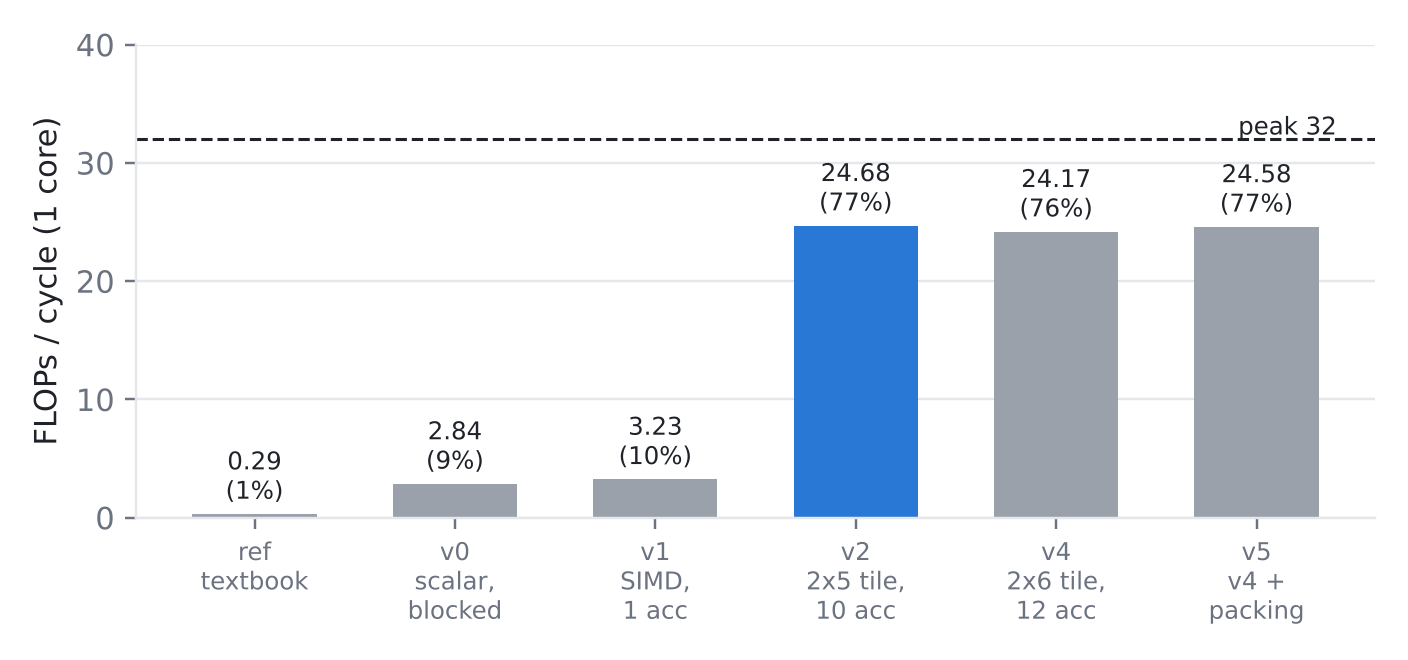
\includegraphics[width=\linewidth]{staircase.png}
\caption{Stride-1 kernel, FLOPs/cycle over all 32 layers, one core.}\label{fig:stair}
\end{minipage}\hfill
\begin{minipage}{0.45\linewidth}\centering
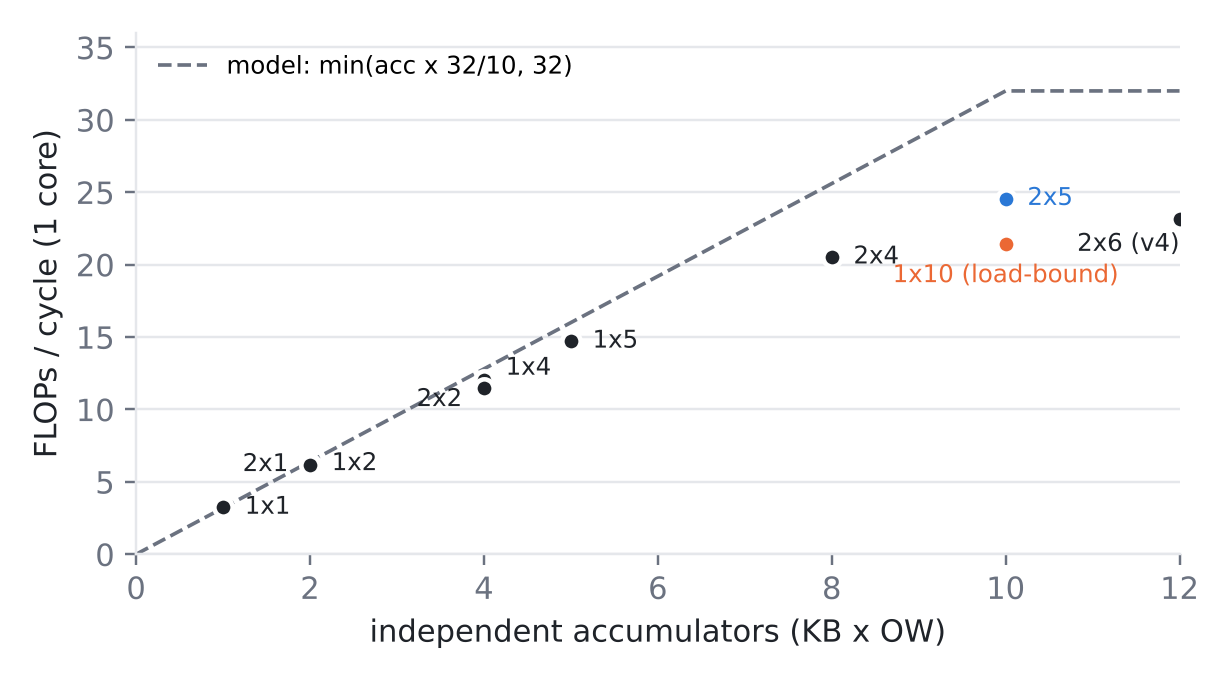
\includegraphics[width=\linewidth]{accumulators.png}
\caption{Same microkernel, different tiles (mean of $C$=16, 32, 64, 128 layers).}\label{fig:acc}
\end{minipage}
\end{figure}

\textbf{Accumulators} (Figure~\ref{fig:acc}). Throughput rises by $\approx$3.2 FLOPs/cycle per accumulator, 90--101\% of the latency model up to 5, then bends to 80\% of the model at 8 and 77\% at 10. 1$\times$10 has 10 accumulators too but 11 loads per 10 FMAs and drops to 21.4: the register-reuse argument, measured.

\textbf{Where the last 23\% goes.} Counters on the $C=64$ layer (v2, 1{,}000 runs): 2.95 uops issued per cycle of 4, so not the front end; ports 0 and 1 busy 80--81\% of cycles with almost only FMAs (7.75\,G uops for 7.39\,G FMAs); allocation stalled 24\% of cycles, half on a full scheduler, none on ROB or store buffer. The scheduler fills with FMAs waiting on their running sums, so the next steps' broadcast loads cannot enter early and their latency shows. That is why \textbf{v4} (2$\times$6, 12 accumulators, row tails; 24.17--24.49) and \textbf{v5} (v4 plus weights repacked in reading order; 24.58) did not help. Next: software pipelining (issue loads a step ahead), as BLIS does in assembly.

\textbf{Multi-core.} v3 on 20 threads runs the 32 layers in 5.15\,ms vs 69.5\,ms on one core (13.5$\times$, 1{,}127 GFLOP/s, 73\% of the 20-core peak at base clock; most layers 75--83\%). Two layers stay near 50\% in two separate runs while same-shape neighbours reach 80\%; the likely cause is that one thread first-touches all buffers, placing them on one socket, which NUMA-aware allocation is next to test.

\subsection{3$\times$3 stride-2 microkernel (O'Malley)}
\todo{O'Malley}{Answer (a)--(e) for your kernel the way the stride-1 subsection does: (a) outputs per call; (b) registers needed vs 16; (c) which register holds what; (d) reuse per register; (e) loop order, unrolling and threading, with pseudo-code. If you reuse the 2$\times$5 tile, say what changes (input column $2(w{+}j){+}s$, row $2h{+}r$, so broadcasts step by $2\cdot8$ floats) and why it still fits every width (320, 160, 80, 40, 20) and every $K/8$. Then your measured versions (\code{scripts/run\_kernels.sh s2\_vN 3x3s2}): FLOPs/cycle and \% of peak per version, what bottleneck each removed, and how you handled the stem.}

\subsection{1$\times$1, SPPF and SiLU (Simon)}
\todo{Simon}{(a)--(e) for the 1$\times$1 microkernel: it is a GEMM tile (the stride-1 template with $R=S=1$ works; note the 1-pixel input halo means reading starts at (row+1, col+1)); weight slab for two output blocks is 24--32\,KB at $C=384/512$, right at the 32\,KB L1. Then SPPF: separable 5$\times$5 max (1$\times$5 then 5$\times$1), $-\infty$ border (the SiLU output feeding SPPF is negative 9\% of the time, so a zero halo would be wrong), pools written straight into their slice of the 512-channel buffer. Then SiLU: the \code{vdivps} vs \code{vrcpps}+Newton change and its measured effect on all three kernels. Measured numbers for each.}

% ===========================================================================
\section{Memory hierarchy design}\label{sec:mem}
An intermediate layout \emph{is} required: ONNX's plain NCHW/OIHW layouts give the microkernels neither contiguous 8-channel vectors nor branch-free borders. We use \textbf{one layout for all three kernels} (\code{include/common.h}), so layers chain with no conversion; conversions happen only at the network input and output.
\begin{itemize}
\item \textbf{Activations: NCHW8c with a halo,} \code{[N][C/8][H+2][W+2][8]}. The 8 innermost floats are 8 consecutive channels, one register. The 1-pixel zero border stores the padding explicitly, so every microkernel call is identical. Each kernel writes only the interior of its output, so the next layer reads it directly.
\item \textbf{Weights,} packed offline like BatchNorm folding: \code{[K/8][C/8][R][S][8 in][8 out]}. The stride-1 v5 variant interleaves the two output blocks of a tile, \code{[K/16][C/8][3][3][8 in][2][8 out]}, so its microkernel reads one stream in order.
\item \textbf{Free Split and Concat.} In NCHW8c each 8-channel block is its own plane, so the C2f \emph{Split} is a pointer offset and \emph{Concat} is the producer writing into its slice of a larger buffer.
\item \textbf{Stride-1 working set (Om).} Per tile pair the weight slab is $576C$ bytes: 9, 18, 37, 74, 147\,KB for $C$ = 16, 32, 64, 128, 256 against a 32\,KB L1 and 256\,KB L2. It is reused across a whole output plane, so even L2-resident slabs keep 73--80\%; only the two $C=256$ head layers (67--71\%), whose weights and 400\,KB input both exceed L2, lose noticeably. Input-channel blocking (or a Morton-ordered traversal of output tiles) for them is future work.
\end{itemize}
\todo{O'Malley}{Working set and access pattern of the stride-2 kernel in this layout: does the stride-2 read of every other input column waste half of each cache line, and does an even/odd column split (an intermediate layout only for its input) pay off? Size of the \code{model.0}/\code{model.1} inputs vs L2/L3.}
\todo{Simon}{Working set of the 1$\times$1 kernel (weights up to 512$\times$256 floats = 512\,KB, exceeds L2) and whether it needs input-channel blocking; the SPPF buffers with a 2-pixel $-\infty$ halo, and writing the pools into slices of the concat buffer.}

% ===========================================================================
\section{Performance baseline}
Both baselines run the same ONNX model on the same images, single-threaded, timed per layer (OpenCV DNN \code{getPerfProfile}, ONNX Runtime profiler; \code{scripts/baseline\_bench.py}). Their FLOPs/cycle use the measured 3.39\,GHz core clock, so they are in real cycles like ours. Data type: FP32 only.

\textbf{3$\times$3 stride 1 (Om)} (Figure~\ref{fig:base}, the 11 distinct layer shapes).
\begin{figure}[H]\centering
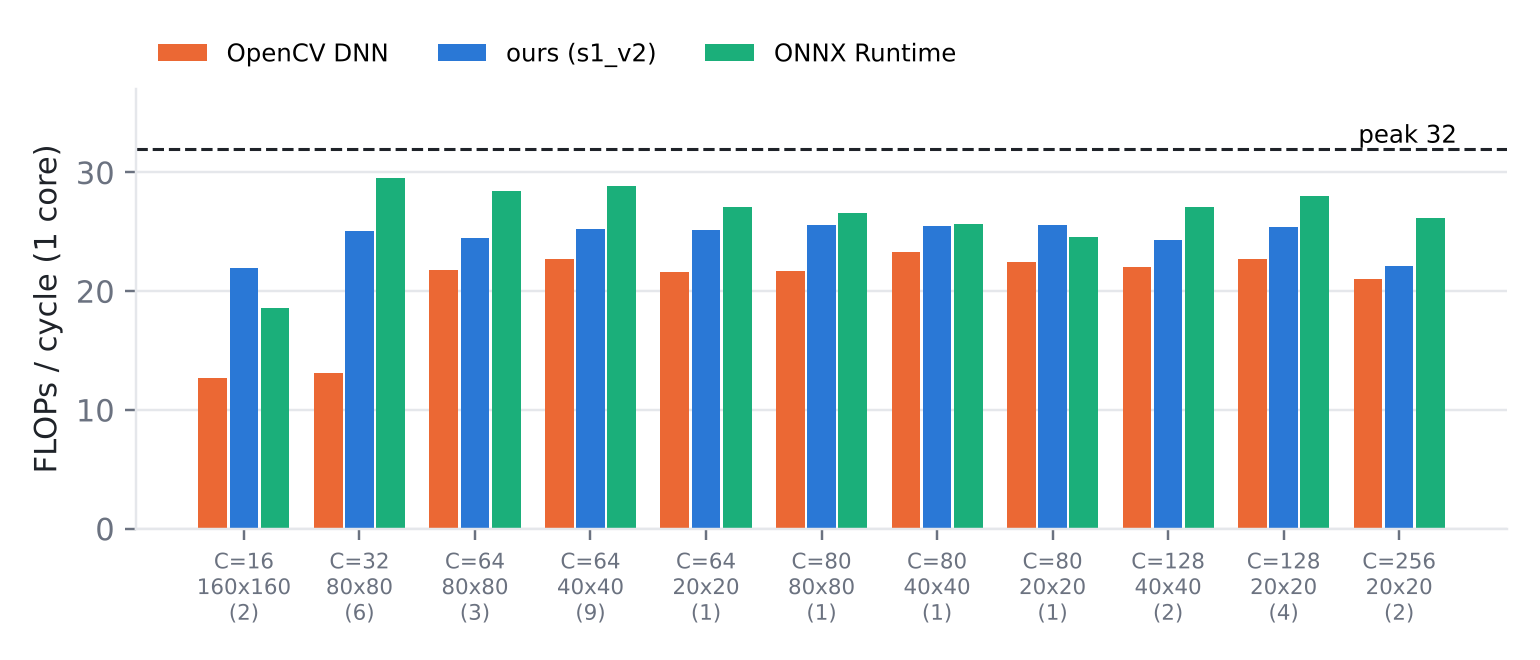
\includegraphics[width=0.86\linewidth]{layers_vs_baselines.png}
\caption{Stride-1 layers: FLOPs/cycle per layer shape (number of layers in parentheses), one core. Dashed line: 32 FLOPs/cycle peak.}\label{fig:base}
\end{figure}
\begin{itemize}
\item \textbf{Baselines vs peak.} OpenCV DNN: 19.8 FLOPs/cycle overall (\textbf{62\%}), 12.7--23.3 per layer, about 40\% on the $C\le32$ layers. ONNX Runtime: 27.4 (\textbf{86\%}), 18.6--29.7.
\item \textbf{Ours vs peak.} 24.7 (\textbf{77\%}), 21.3--25.8, the most uniform of the three: on the $C=16$, 160$\times$160 layers 69\% vs 58\% (ONNX Runtime) and 40\% (OpenCV). Total for the 32 layers: 69.5\,ms ours, 86.4\,ms OpenCV DNN, 62.6\,ms ONNX Runtime.
\end{itemize}

\todo{O'Malley}{Same for the 7 stride-2 layers: \code{python docs/milestone/om/make\_figs.py} shows how the figure is made from \code{results/s2\_vN\_b1\_t1.csv} and \code{results/baseline\_b1\_t1.csv}; give baseline and your \% of peak.}
\todo{Simon}{Same for the 24 1$\times$1 layers, and SPPF/SiLU timings against the baselines' MaxPool and Sigmoid+Mul nodes.}

\textbf{Summary and next steps.}
\todo{All}{One table: per kernel, best version, \% of peak on 1 core, baseline \% of peak, 20-core speedup. Then the next phase: chaining all kernels into the full network and timing it end to end, NUMA-aware threading, batch 16.}
Stride-1 next steps: a software-pipelined microkernel for the last $\approx$20\%, cache blocking for the $C=256$ layers, NUMA-aware threading, and batch 16.

\end{document}
